% Documento principal del informe
\documentclass{article}
\usepackage[utf8]{inputenc}
\usepackage{graphicx}
\usepackage[spanish,es-tabla]{babel}
\usepackage{amsmath}
\usepackage[a4paper,margin=1in]{geometry}
\usepackage{subcaption}
\usepackage{amssymb}
\usepackage[hidelinks]{hyperref}
\usepackage{mathtools}
\usepackage[table,xcdraw]{xcolor}
\usepackage[backend=bibtex]{biblatex}
\usepackage{csquotes}
\usepackage{lipsum} % Generar texto de muestra (puedes eliminarlo después)
\usepackage{caption}
\usepackage{amsmath}
\usepackage{enumitem}
\usepackage{listings}
\usepackage{xcolor} % Paquete para manejar colores
\usepackage{float} % Necesario para utilizar la opción [H]

\addbibresource{bibliografia.bib} %archivo de bibliografia

\begin{document}

\renewcommand{\figureautorefname}{Fig.}
\renewcommand{\tableautorefname}{Tab.}
\renewcommand{\equationautorefname}{Ec.}

\begin{titlepage}

    \thispagestyle{empty}
    
    % Portada Custom, ver /maketitle: https://www.overleaf.com/learn/latex/How_to_Write_a_Thesis_in_LaTeX_(Part_5)%3A_Customising_Your_Title_Page_and_Abstract
    
    \begin{center}
        
\includegraphics[width=5cm]{figures/unc_logo.png} \hspace{2cm}
        
\includegraphics[width=5cm]{figures/fcefyn_logo.jpg}
        \\[1cm]
        \vspace{5pt}
        \LARGE Universidad Nacional de Córdoba\\[0.5cm] 
        \large Facultad de Ciencias Exactas, Físicas y Naturales \\[0.5cm] 
        \large Electrónica Analógica III
        \\[0.2cm]
        \large Trabajo Práctico N° 1
        \\[0.2cm]
        \vspace{60pt}
        \begin{table}[!h]
        \centering
        \begin{tabular}{ll}
        \multicolumn{1}{c}{Nombre} & \multicolumn{1}{c}{DNI} \\
        Clemenz Jeremías & 43449566 
        \end{tabular}
        \end{table}
        \vspace{20pt}
        \begin{table}[!h]
        \centering
        \begin{tabular}{ll}
        \multicolumn{1}{c}{Docentes} & Ing. Rodrigo Bruni \\
         & Ing. José Amado \\
         & Ing. Federico Dadam
        \end{tabular}
        \end{table}
        \vfill
        Córdoba, República Argentina\\
        \today
    \end{center}
    
    \end{titlepage}
\newpage

\tableofcontents
\newpage
\listoffigures
\newpage
\listoftables

\newpage

\section{Introducción}

En el trabajo practico N° 1 se realizara el estudio de un circuito de acoplamiento interetapas. Los circuitos interetapa se utilizan en sistemas 
de comunicacion para adaptar impedancia y sintonizar en una frecuencia determinada, permitiendo maxima transferencia de energia entre etapas.
En el practico construiremos el circuito resonante, armando la bobina y utilizando capacitores comerciales, donde tendremos que cumplir valores de frecuencia central, ancho 
de banda, factor de calidad e impedancia de entrada y salida.

HOLA HOLA 


\newpage
\section{Marco teórico}

\subsection{Circuito resonante RLC}

Un circuito resonante está compuesto por una resistencia, bobina y un capacitor (Figura 1), en el cual se produce una resonancia en una frecuencia determinada. La frecuencia de resonancia es aquella en 
la cual la reactancia inductiva y la reactancia capacitiva son iguales, por lo que la impedancia del circuito es puramente resistiva. 

\begin{figure}[h]
    \centering
    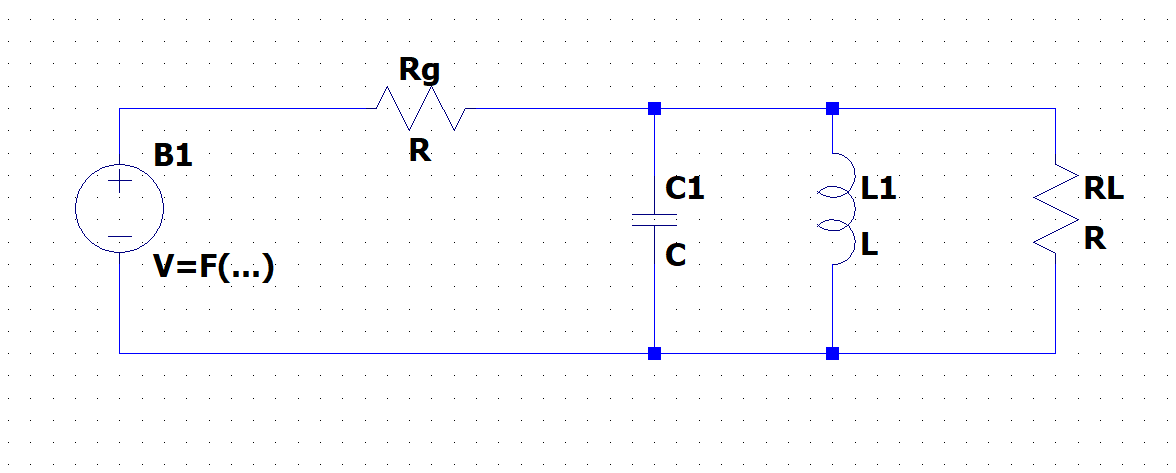
\includegraphics[width=0.5\textwidth]{Imagenes/circuito_resonante.png}
    \caption{Circuito resonante RLC}
    \label{fig:circuito_resonante}
\end{figure}

La frecuencia de resonancia o frecuencia central ($f_0$) caracteriza al circuito resonante, y se calcula mediante la siguiente ecuación:

\begin{equation}
    f_0 = \frac{1}{2\pi \sqrt{LC}}
\end{equation}

Donde: 
\begin{itemize}
    \item $f_0$ es la frecuencia central
    \item $L$ es la inductancia
    \item $C$ es la capacidad
\end{itemize}

En la última ecuación podemos observar que la frecuencia central depende de la inductancia $L$ y la capacidad $C$. 
A partir de la $f_0$ podemos definir el factor de calidad cuando el circuito está cargado ($Q_c$) y cuando el circuito está descargado ($Q_d$). 
Se pueden calcular mediante las siguientes ecuaciones:

\begin{equation}
    Q_c = \frac{f_0}{BW} = \frac{R_T}{X_L}
\end{equation}

\begin{equation}
    Q_d = \frac{R_P}{X_L}
\end{equation}

Donde: 

\begin{itemize}
    \item $R_T$ es la resistencia total
    \item $R_P$ es la resistencia paralelo
    \item $X_L$ es la reactancia inductiva
    \item $BW$ es el ancho de banda
\end{itemize}

La variable $R_T$ es la resistencia total del circuito, la cual determinará el factor de calidad cargado del circuito. 
El inductor real tendrá pérdidas parasitarias, esta resistencia se encuentra en paralelo con el inductor
de la figura 1 y se denomina resistencia en paralelo ($R_P$). La resistencia total del circuito $R_T$ se calcula mediante la siguiente ecuación:

\begin{equation}
    R_T = R_P \parallel R_L \parallel R_g
\end{equation}

Donde:
\begin{itemize}
    \item $R_P$ es la resistencia paralelo
    \item $R_L$ es la resistencia de carga
    \item $R_g$ es la resistencia del generador
\end{itemize}

En este trabajo práctico se pretende diseñar un circuito resonante a una determinada frecuencia central y ancho de banda. Por lo tanto realizaremos una 
modificación del circuito de la figura 1, para obtener el circuito de acoplamiento interetapas (Figura 2). 

\begin{figure}[h]
    \centering
    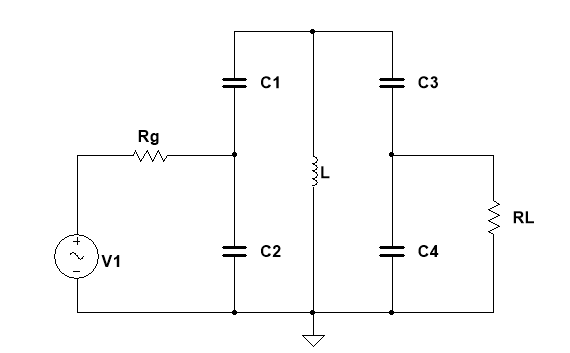
\includegraphics[width=0.5\textwidth]{Imagenes/circuito_acoplamiento2.png}
    \caption{Circuito de acoplamiento interetapas RLC modificado}
\end{figure}

El circuito de la figura 2 tiene la misma frecuencia central que el circuito de la figura 1. Si calculamos la capacidad total, obtendremos la misma que la del circuito de la figura 1.

\begin{equation}
    C_T = \frac{C1 \cdot C2}{C1 + C2} + \frac{C3 \cdot C4}{C3 + C4} = \frac{C}{2} + \frac{C}{2} 
\end{equation}

Analizando la salida del circuito de la figura 2, podemos trazar un paralelismo con el autotransformador, donde podemos reflejar las impedancias tanto del 
generador como de la carga al primario. Y donde cada capacitor o la suma de ellos es el bobinado del autotransformador.

\begin{figure}[h]
    \centering
    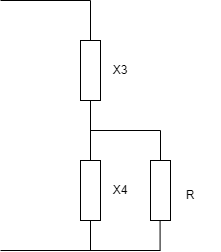
\includegraphics[width=0.3\textwidth]{Imagenes/Esquema_autotrafo.png}
    \caption{Autotransformador}
\end{figure}

Del autotransformador podemos obtener la relación de transformación:

\begin{figure}[h]
    \centering
    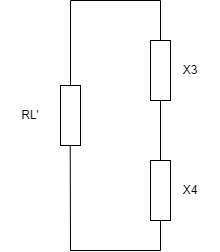
\includegraphics[width=0.3\textwidth]{Imagenes/relacion_transformacion.png}
    \caption{Esquema de relación de transformación}
\end{figure}

\begin{equation}
    R_L' = (1 + \frac{C_3}{C_4})^2 \cdot R_L 
\end{equation}

\begin{equation}
    R_g' = (1 + \frac{C_1}{C_2})^2 \cdot R_g
\end{equation}

Finalmente, el circuito reflejado de la figura 2 queda como se muestra en la figura 5:

\begin{figure}[h]
    \centering
    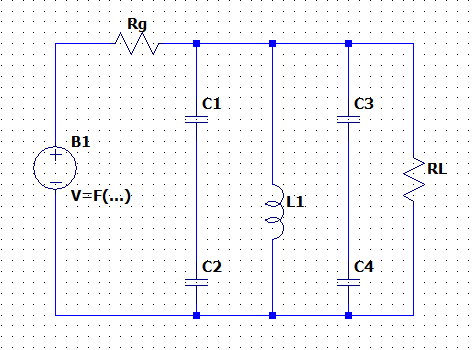
\includegraphics[width=0.5\textwidth]{Imagenes/circuito_reflejado.png}
    \caption{Circuito reflejado}
\end{figure}

Donde nos queda una resistencia total de:

\begin{equation}
    R_T = R_g' \parallel R_L' \parallel R_P
\end{equation}

Donde:

\begin{itemize}
    \item $R_g'$ es la resistencia del generador reflejada
    \item $R_L'$ es la resistencia de carga reflejada
    \item $R_P$ es la resistencia paralelo
\end{itemize}

Con el circuito reflejado, las resistencias $R_g'$ y $R_L'$ dependerán de los capacitores $C1$, $C2$, $C3$ y $C4$, lo que nos permitirá adaptar las impedancias de entrada y salida del circuito.
Podemos realizar la siguiente asignación de valores, donde seguiremos cumpliendo la condición de la ecuación 7:

\begin{equation}
    R_T = X_L \cdot Q_c = R_g' \parallel (R_L' \parallel R_P) = 2 R_T \parallel 2 R_T 
\end{equation}

Finalmente, luego de este desarrollo nos quedará un sistema de ecuaciones con 4 incógnitas, las cuales son $C1$, $C2$, $C3$ y $C4$, que nos servirán para el diseño del circuito de acoplamiento.

\begin{equation}
    \begin{cases}
        R_L' = \left(1 + \frac{C_3}{C_4}\right)^2 \cdot R_L \vphantom{\frac{C_1 \cdot C_2}{C_1 + C_2}} \\
        \\
        R_g' = \left(1 + \frac{C_1}{C_2}\right)^2 \cdot R_g \vphantom{\frac{C_1 \cdot C_2}{C_1 + C_2}} \\
        \\
        \frac{C_1 \cdot C_2}{C_1 + C_2} = \frac{C}{2} \\
        \\
        \frac{C_3 \cdot C_4}{C_3 + C_4} = \frac{C}{2}
    \end{cases}
\end{equation}

\subsection{Condición para la reflexión de impedancias}

La demostración de la reflexión de impedancias se parte de un circuito mixto y se lo lleva a otro paralelo. En la siguiente figura se muestran la forma que queremos expresar el circuito.

\begin{figure}[h]
    \centering
    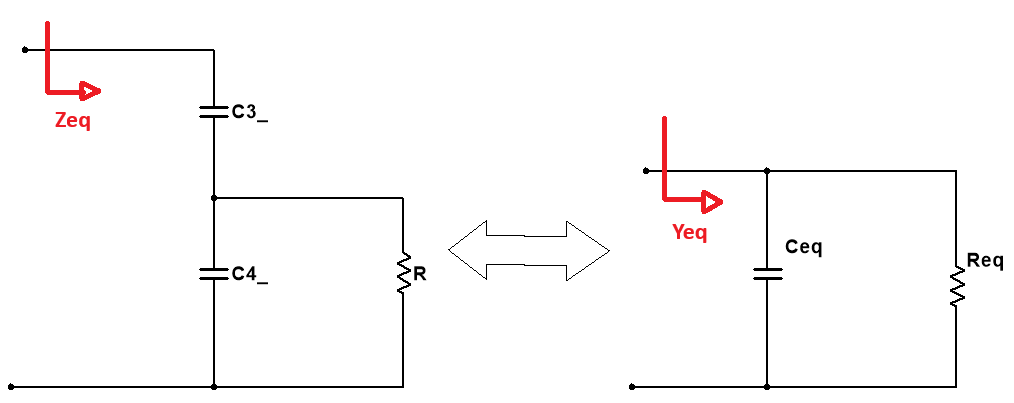
\includegraphics[width=0.8\textwidth]{Imagenes/reflexion_impedancias.png}
    \caption{Circuitos equivalentes}
\end{figure}

La impedancia equivalente del circuito mixto se puede expresar como:

\begin{equation}
    Z_{eq} = X_{C3} + X_{C4} // R 
\end{equation}

Desarrollando la ecuación anterior, obtenemos:

\begin{equation}
    Z_{eq} = \frac{R \cdot (1 + \frac{C4}{C3}) - j \cdot \frac{1}{2 \pi f C3}}{1 + j \cdot R \cdot 2 \pi f C4} 
\end{equation}

Luego para pasar al modelo equivalente paralelo podremos expresar la impedancia como admitancia para mayor facilidad de cálculo:

\begin{equation}
    Y_{eq} = \frac{1}{Z_{eq}} = \frac{1 + j \cdot R \cdot 2 \pi f C4}{R \cdot (1 + \frac{C4}{C3}) - j \cdot \frac{1}{2 \pi f C3}}
\end{equation}

Racionalizando la expresión:

\begin{equation}
    Y_{eq} =  \frac{1}{Z_{eq}} = \frac{1 + j \cdot R \cdot 2 \pi f C4}{R \cdot (1 + \frac{C4}{C3}) - j \cdot \frac{1}{2 \pi f C3}} \cdot \frac{R \cdot (1 + \frac{C4}{C3}) + j \cdot \frac{1}{2 \pi f C3}}{R \cdot (1 + \frac{C4}{C3}) + j \cdot \frac{1}{2 \pi f C3}}
\end{equation}

Finalmente, obtenemos la expresión de la admitancia equivalente:

\begin{equation}
    Y_{eq} = \frac{R + j \cdot (2 \pi)^2 \cdot f^2 \cdot C4 \cdot (1 + \frac{C4}{C3})}{R^2 \cdot (1 + \frac{C4}{C3})^2 + \frac{1}{4 \pi^2 f^2 C3^2}}
\end{equation}

Tomando la parte real de la admitancia para obtener la conductancia equivalente:

\begin{equation}
    G_{eq}= Re(Y_{eq}) = \frac{R}{R^2 \cdot (1 + \frac{C4}{C3})^2 + \frac{1}{4 \pi^2 f^2 C3^2}}
\end{equation}

Simplificando e invirtiendo la expresión, obtenemos la $R_{eq}$ que es la resistencia equivalente del circuito paralelo que inicialmente queremos:

\begin{equation}
    R_{eq} = R \cdot (1 + \frac{C4}{C3})^2 + \frac{1}{R \cdot 4 \pi^2 f^2 C3^2}
\end{equation}

El segundo término de la ecuación 17 hace que no se cumpla la reflexión de impedancias. Para solucionar este problema, se debe cumplir la siguiente condición:

\begin{equation}
    R \cdot 4 \pi^2 f^2 C3^2 \gg 10 
\end{equation}

El parámetro que podremos variar para cumplir la condición de la ecuación 18 es la capacidad de C3. 


\newpage
\section{Desarrollo}

\subsection{Rerequerimientos}

Para este trabajo practico se nos solicita realizar un circuito resonante que cumpla con las siguientes especificaciones:

\begin{itemize}
    \item Frecuencia de resonancia: $f_0 = 16 MHz$
    \item Ancho de banda: $BW = 1.6 MHz$
    \item Factor de calidad con el circuito cargado: $Q_c = 10$
    \item Impedancia de entrada: $Z_{in} = 50 \Omega$
    \item Impedancia de salida: $Z_{out} = 1 k\Omega$
\end{itemize}

\subsection{Diseño}

El primer paso para construir el circuito resontate es realizar los calculos del inductor. Para ello, se utilizara la siguiente formula:

% L = D^3 * Ns^2 k 10^-3 [micro H]
\begin{equation}
    L = D^3 \cdot N_s^2 \cdot k \cdot 10^{-3}\; [\mu F]
\end{equation}

Donde:

\begin{itemize}
    \item $D$ es el diametro externo del inductor en cm 
    \item $N_s$ es el numero de espiras por unidad de longitud en espiras/cm
    \item $k$ es la constante que depende de la relacion de longitud con diametro l/D
\end{itemize}

Para comenzar fijaremos parametros que podamos ajustarlos o determinarlos. Elegimos los siguientes valores:

\begin{itemize}
    \item $D =  2.21\; \text{cm}$
    \item diametro del conductor: $d = 2.1\; \text{mm}$
    \item separacion entre espiras: : $S = 3\; \text{mm}$
\end{itemize}

Con estos valores, se puede calcular el numero de espiras por unidad de longitud:

\begin{equation}
    N_s = \frac{1}{S + d} = \frac{10}{3 + 2.1 } = 2\; \text{espiras/cm}
\end{equation}

Para seguir con los calculos necesitaremos seleccionar un valor de longitud del inductor $L$. En la planilla de calculo se definieron valores de longitud con un paso de 0.1 cm.
Finalmente seleccionamos:

% separar unidad de numero 
\begin{itemize}
    \item $L = 3.8\; \text{cm}$
\end{itemize}

Calculamos la cantidad de espiras:

\begin{equation}
    N = N_s \cdot L = 2 \cdot 3.8 = 7\; \text{espiras} 
\end{equation}

Tenemos que tener en cuenta que redondeamos para Ns de 1.96 a 2. Ahora calculamos la relacion de longitud con diametro:

\begin{equation}
    \frac{L}{D} = \frac{3.8}{2.21} = 1.72
\end{equation}

Ahora tendremos que calcular la constante de Nagaoka, para esto hay dos formas de hacerlo. La primera es mediante la siguiente formula:

% k = K * Pi ^2 * L/D
\begin{equation}
    k = K \cdot \pi^2 \cdot \frac{L}{D} 
\end{equation}

Donde $K$ se calcula mediante la siguiente formula:

% K = 1 / (1 + 0.9 D/2L - 2*10^-2 (D/2L)^2)
\begin{equation}
    K = \frac{1}{1 + 0.9 \cdot \frac{D}{2L} - 2 \cdot 10^{-2} \left(\frac{D}{2L}\right)^2}
\end{equation}

Sustituyendo los valores obtenemos:

\begin{equation}
    K = \frac{1}{1 + 0.9 \cdot \frac{2.21}{2 \cdot 3.8} - 0.2 \cdot 10^{-2} \left(\frac{2.21}{2 \cdot 3.8}\right)^2} = 0.79
\end{equation}

Y el factor de Nagaoka:

\begin{equation}
    k = 0.79 \cdot \pi^2 \cdot 1.72 = 13.5
\end{equation}

La otra forma es graficamente, donde con L/D = 1.72 ingresamos al siguiente grafico:

\begin{figure}[h]
    \centering
    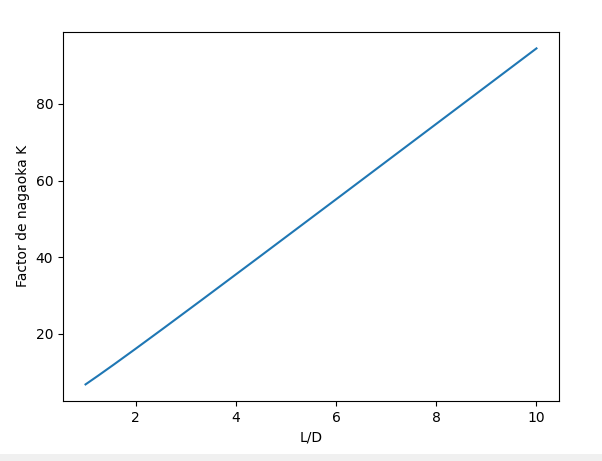
\includegraphics[width=0.5\textwidth]{Imagenes/factorNagaoka.png}
    \caption{Curva de Nagaoka K}
\end{figure}

Donde obtendremos un valor aproximado de forma grafica.

Con todos estos parametros calculados, podemos calcular el valor de la inductancia:

\begin{equation}
    L = D^3 \cdot N_s^2 \cdot k \cdot 10^{-3} = 2.21^3 \cdot 2^2 \cdot 13.5 \cdot 10^{-3} = 0.56\; \mu H
\end{equation}

\subsubsection{Calculo de resistencias}

Para el calculo de las resistencias necesitaremos calcular el factor de calidad sin carga $Q_d$, con la siguiente formula:

\begin{equation}
    Q_d = 8850 \cdot \frac{D \cdot L}{102 \cdot L + 45 \cdot D} \cdot \sqrt{f_0}
\end{equation}

Donde:

\begin{itemize}
    \item $L$ es la longitud del inductor en cm
    \item $D$ es el diametro del inductor en cm
    \item $f_0$ es la frecuencia de resonancia en MHz
\end{itemize}

Sustituyendo los valores obtenemos:

\begin{equation}
    Q_d = 610.4 
\end{equation}

La reactancia del inductor es:

\begin{equation}
    X_L = 2 \cdot \pi \cdot f_0 \cdot L = 2 \cdot \pi \cdot 16 \cdot 10^6 \cdot 0.56 \cdot 10^{-6} = 56\; \Omega
\end{equation}

Con $X_L$ y $Q_d$ podemos calcular la resistencia paralela $R_p$:

\begin{equation}
    R_p = Q_d \cdot X_L = 610.4 \cdot 56 = 34300\; \Omega
\end{equation}

Con $Q_C$ y $X_L$ podemos calcular la resistencia total $R_t$:

\begin{equation}
    R_t = \frac{X_L}{Q_c} = \frac{56}{10} = 560\; \Omega
\end{equation}

Con los valores calculados podremos calcular la resistencia de carga reflejada $R_L'$ y la resistencia del generador reflejada $R_g'$, para esto tenemos que despejar $R_L'$ y $R_g'$ de la ecuacion 8:

\begin{equation}
    R_L' // R_P = 2 \cdot R_T 
\end{equation}

\begin{equation}
    R_g' = 2 \cdot R_T 
\end{equation}

Despejando $R_L'$ obtenemos:

\begin{equation}
    R_L' = \frac{2 \cdot R_T \cdot R_P}{R_P - 2 \cdot R_T} 
\end{equation}

Sustituyendo los valores obtenemos:

\begin{equation}
    R_L' = \frac{2 \cdot 560 \cdot 34300}{34300 - 2 \cdot 560} = 1161.8\; \Omega
\end{equation}

Y calculando $R_G'$:

\begin{equation}
    R_g' = 2 \cdot 560 = 1123\; \Omega
\end{equation}


% subsection de la subsection de diseño
\subsubsection{Calculo del capacitor}

Con la frecuencia de resonancia $f_0 = 16 MHz$ y el valor de la inductancia calculado, podemos calcular el valor del capacitor:

\begin{equation}
    C = \frac{1}{L \cdot (2 \cdot \pi \cdot f_0)^2} = \frac{1}{0.56 \cdot (2 \cdot \pi \cdot 16 \cdot 10^6)^2} = 177\; \text{pF}
\end{equation}

Con las ecuaciones del sistema de ecuaciones 13, podemos calcular $C_1$, $C_2$, $C_3$ y $C_4$:

\begin{equation}
    C_2 = \frac{C}{2} \cdot \sqrt{\frac{R_g'}{R_g}}
\end{equation}

Entonces $C_1$ sera igual a: 

\begin{equation}
    C_1 = \frac{C_2}{\sqrt{R_g' / R_g - 1}}
\end{equation}

Con $C_4$ y $C_3$ nos queda:

\begin{equation}
    C_4 = \frac{C}{2} \cdot \sqrt{\frac{R_L'}{R_L}}
\end{equation}

\begin{equation}
    C_3 = \frac{C_4}{\sqrt{R_L' / R_L - 1}}
\end{equation}

Remplazando los valores obtenemos:


\begin{equation}
    C_1 = 112\; \text{pF}
\end{equation}

\begin{equation}
    C_2 = 420\; \text{pF}
\end{equation}

\begin{equation}
    C_3 = 1225\; \text{pF}
\end{equation}

\begin{equation}
    C_4 = 95\; \text{pF}
\end{equation}

\newpage
\subsection{Simulacion}

Para comprobar el correcto funcionamiento de nuestro circuito, se realizo una simulacion en LTSpice. A continuacion se muestra el circuito simulado:

\begin{figure}[h]
    \centering
    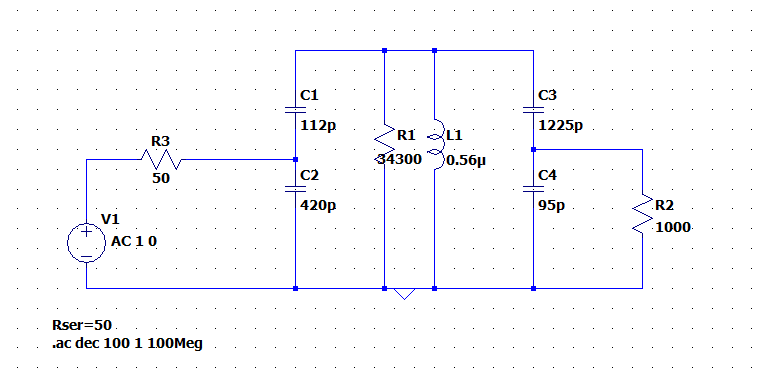
\includegraphics[width=0.7\textwidth]{Imagenes/circuito.png}
    \caption{Circuito simulado en LTSpice}
\end{figure}

La respuesta en frecuencia obtenida del circuito simulada es la siguiente:

\begin{figure}[h]
    \centering
    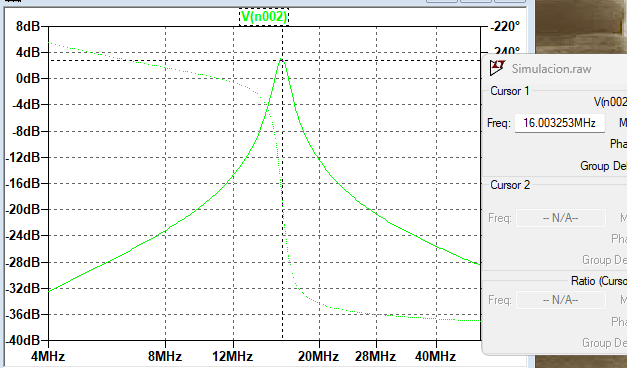
\includegraphics[width=0.7\textwidth]{Imagenes/resultado_circuito.png}
    \caption{Respuesta en frecuencia del circuito simulado}
\end{figure}

Se observa que la frecuencia de resonancia es de $16 MHz$ con una ganancia de $2 dB$. Ademas:

\begin{itemize}
    \item frecuencia de corte inferior: $15.2 MHz$
    \item frecuencia de corte superior: $16.8 MHz$
    \item ancho de banda: $1.6 MHz$
    \item $Q_c = 10$
\end{itemize}

\newpage
\subsection{Seleccion de componentes y armado}

El primer paso sera determinar que capacitores utilizaremos para el circuito. Los capacitores seleccionados son:

\begin{itemize}
    \item $C_1 = 100\; \text{pF}$
    \item $C_2 = 330 + 100 = 430\; \text{pF}$
    \item $C_3 = 1000 + 100 + 100 =1200\; \text{pF}$
    \item $C_4 = 100\; \text{pF}$
\end{itemize}

La capacidad total sera:

\begin{equation}
    C_T = \frac{C_1 \cdot C_2}{C_1 + C_2} + \frac{C_3 \cdot C_4}{C_3 + C_4} 
\end{equation}

\begin{equation}
    C_T = 173.4 \; \text{pF}
\end{equation}

El resultado obtenido con los capacitores obtenidos, haciendo un analisis de montecarlo:

\begin{figure}[h]
    \centering
    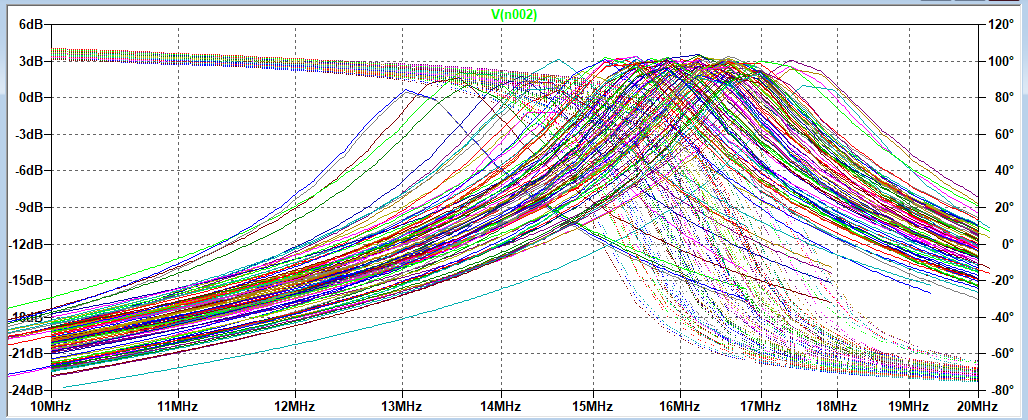
\includegraphics[width=0.7\textwidth]{Imagenes/montecarlo.png}
    \caption{Analisis de montecarlo}
\end{figure}

Vemos que la tolerancia y los capacitores utilizados hace que $f_0$ varie entre $13 MHz y 17.2 MHz$.


El inductor y los capacitores montados en la PCB finalmente nos queda:

\begin{figure}[h]
    \centering
    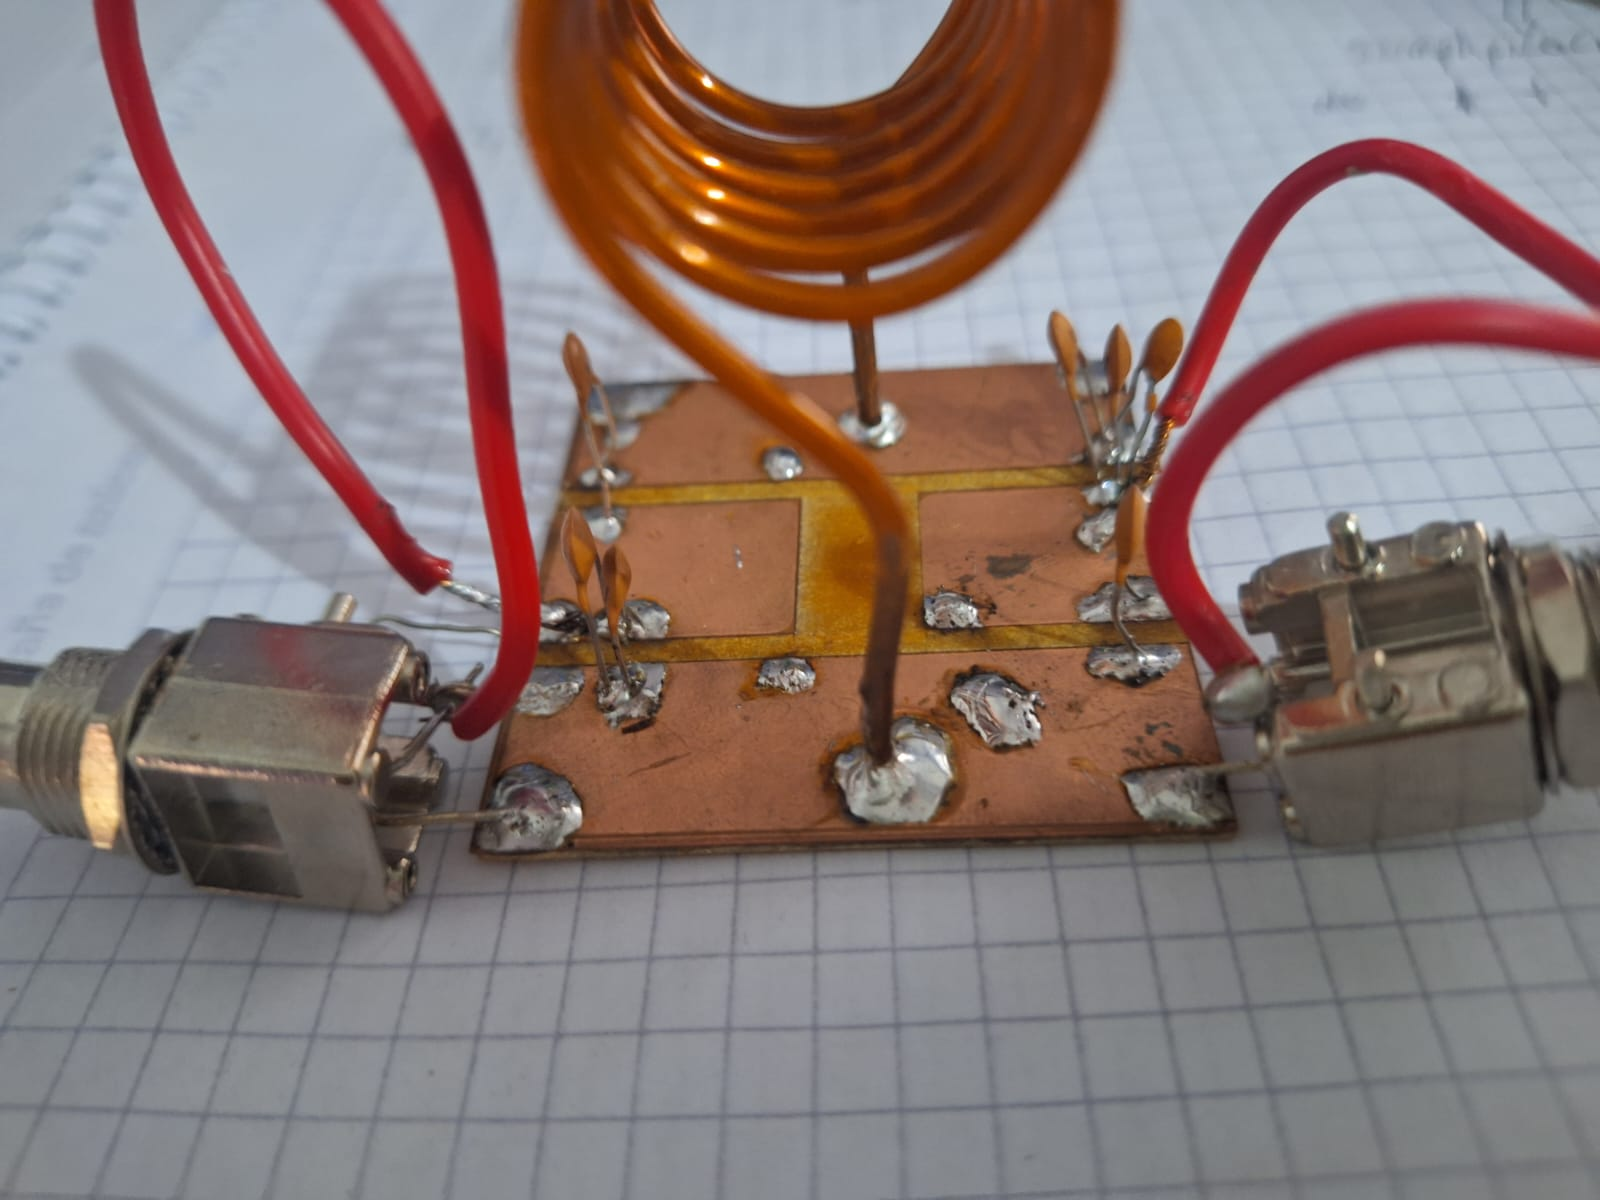
\includegraphics[width=0.7\textwidth]{Imagenes/pcb1.jpeg}
    \caption{PCB montada}
\end{figure}

\begin{figure}[h]
    \centering
    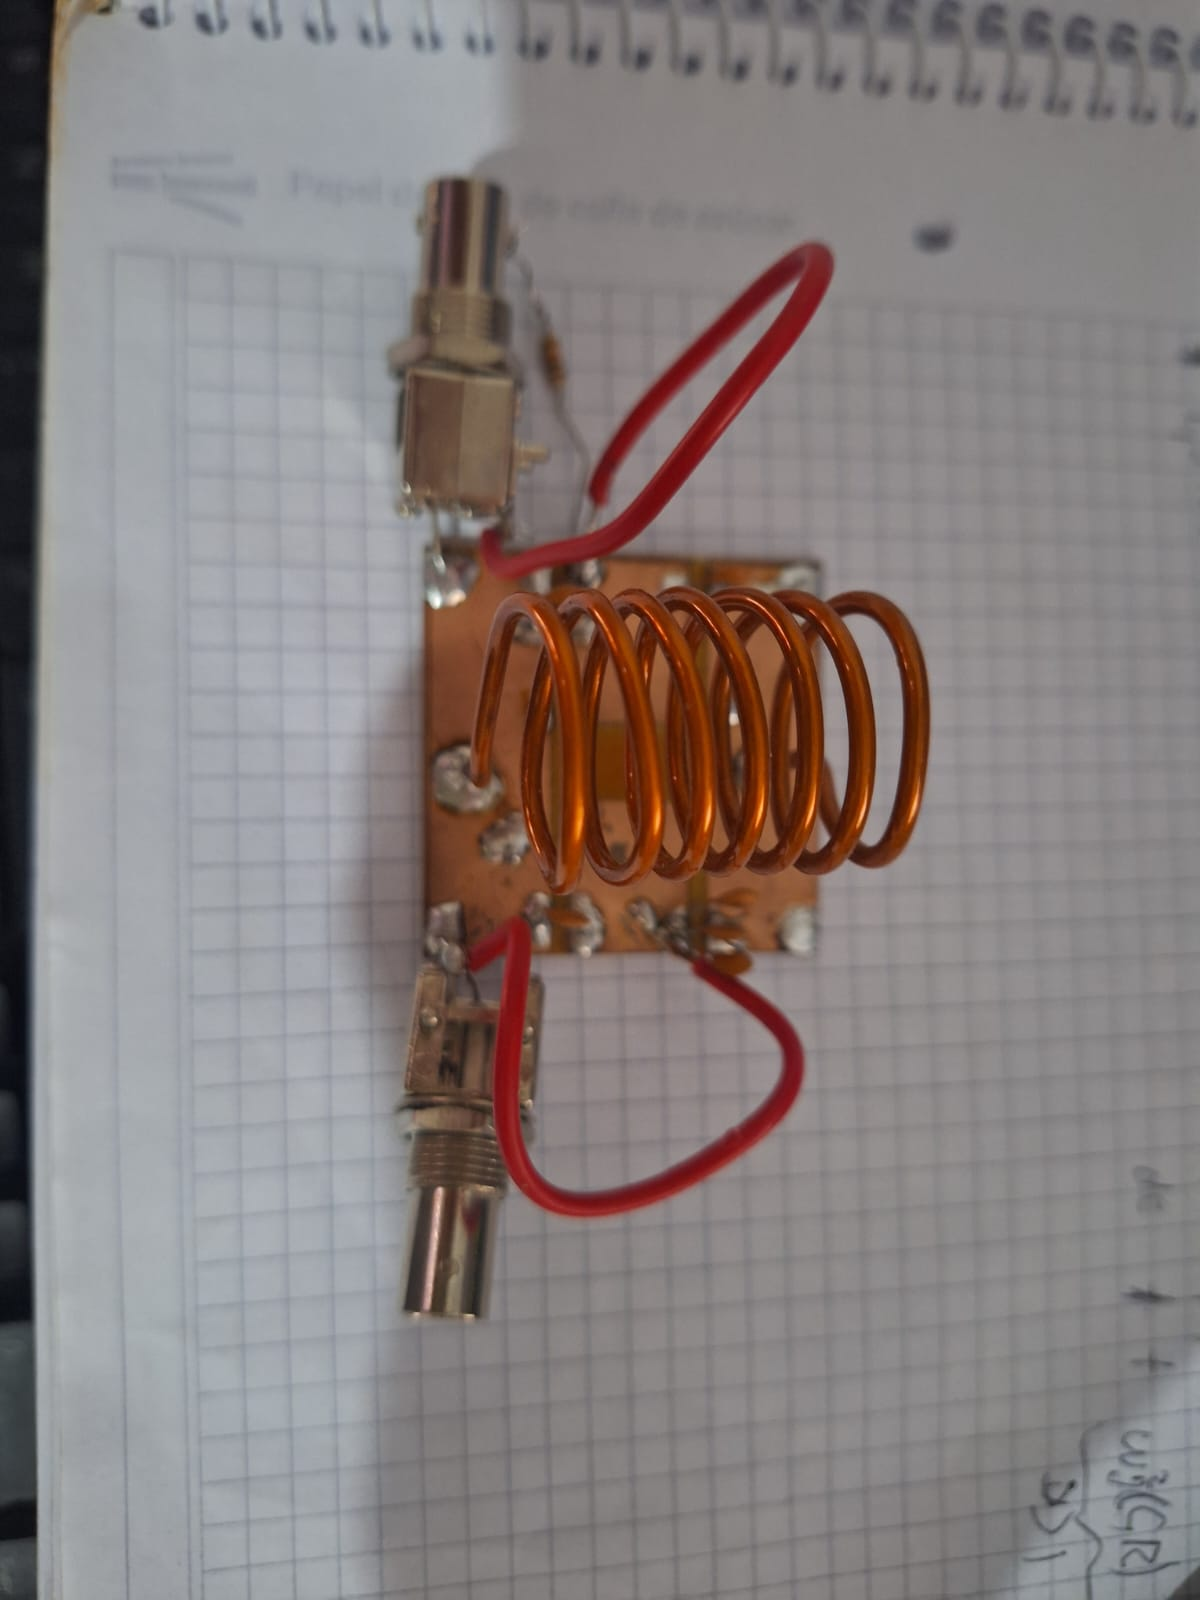
\includegraphics[width=0.7\textwidth]{Imagenes/pcb2.jpeg}
    \caption{PCB montada}
\end{figure}


\subsection{Mediciones}

\subsubsection{Medicion de $f_o$}

Para la medicion de la frecuencia de resonancia, se conecta el circuito a tope. El esquema es el siguiente:

\begin{figure}[h]
    \centering
    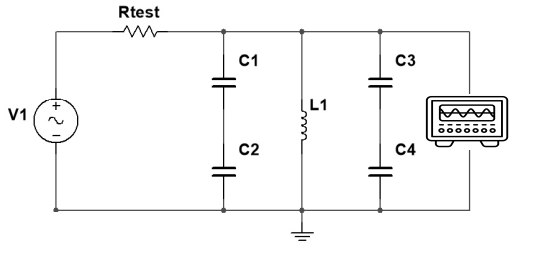
\includegraphics[width=0.5\textwidth]{Imagenes/medicion_fo.png}
    \caption{Medicion de $f_o$}
    \label{fig: de la frecuencia de resonancia $f_o$}
\end{figure}


La resistencia Rtest tiene que ser del orden de  $R_p$, por lo tanto, inicialmente se utilizó una resistencia de 1 k$\Omega$. Una vez realizada la conexión, se varía la frecuencia del generador 
de señales de menor a mayor hasta encontrar la frecuencia de resonancia. Debemos considerar que el osciloscopio tiene una capacidad de entrada, por lo tanto, esta capacidad parásita puede 
afectar la medición de la frecuencia de resonancia.

La medicion $f_o1$:

\begin{equation}
    f_{o1} = 12 MHz 
\end{equation}

A continuacion mediremos la frecuencia de resonancia $f_{o2}$, para esto se utilizara una resistencia de 1k$\Omega$ y ademas, se agrega el capacitor $C_F$ en paralelo al inductor y los capacitores.
El esquema es el siguiente:

\begin{figure}[h]
    \centering
    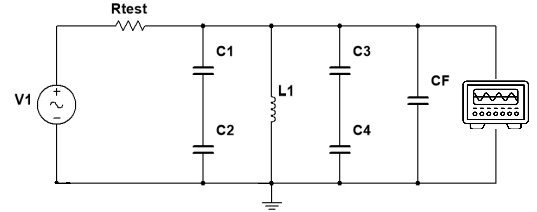
\includegraphics[width=0.5\textwidth]{Imagenes/medicion_fo2.png}
    \caption{Medicion de $f_o2$}
    \label{fig: de la frecuencia de resonancia $f_(o2)$}
\end{figure}

La medicion $f_{o2}$:

\begin{equation}
    f_o2 = 10.5 MHz
\end{equation}

Para obtener la frecuencia de resonancia $f_o$ se debe obtener $C_o$ apartir de estas ecuaciones:

\begin{equation}
    f_o1 = \frac{1}{2\pi\sqrt{L(C_T + C_o)}}
\end{equation}

\begin{equation}
    f_o2 = \frac{1}{2\pi\sqrt{L(C_T + C_o + C_F)}}
\end{equation}

Donde $C_T$ es igual 177 pF. Despejando $C_o$ de estas ecuaciones obtenemos:

\begin{equation}
    (\frac{f_o1}{f_o2})^2 = \frac{C_T + C_o + C_F}{C_T + C_o}
\end{equation}

\begin{equation}
    C_o = \frac{C_T \cdot (f_o2^2 - f_o1^2) + C_F f_o2^2}{f_o1^2 - f_o2^2}
\end{equation}

El capacitor $C_F$ es de 100pF y $C_o$ es de:

\begin{equation}
    C_o = 149,7 pF
\end{equation}

Con este valor, nos damos cuenta de que la capacidad agregada del osciloscopio, cables BNC, soldaduras, etc., es comparable a la del 
circuito, por lo tanto, modificará la medición y afectará el resultado. Ahora determinaremos el valor de la inductancia $L$:

\begin{equation}
    L = \frac{1}{(2\pi f_o1)^2} \cdot \frac{1}{C_T + C_o} = 0.538\; \mu H
\end{equation}

Con este valor determinamos el valor de la frecuencia de resonancia $f_o$:

\begin{equation}
    f_o = \frac{1}{2\pi\sqrt{L \cdot C_T}} = 16.3 MHz
\end{equation}

\subsubsection{Medicion de $BW$}

Para la medicion del ancho de banda, se utiliza el esquema de la figura \ref{fig: de la medicion del ancho de banda}:

% Colocar imagen abajo del texto de arriba
\begin{figure}[h]
    \centering
    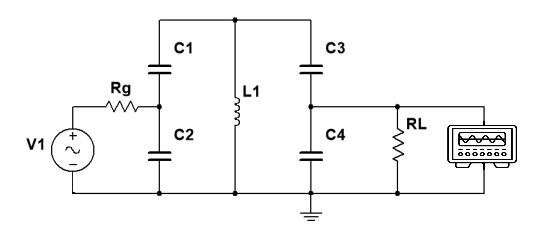
\includegraphics[width=0.5\textwidth]{Imagenes/medicion_bw.png}
    \caption{Medicion de $BW$}
    \label{fig: de la medicion del ancho de banda}
\end{figure}

La medicion del ancho de banda variaremos la frecuencia hasta encontrar el pico maximo de amplitud en la salida, una vez encontrado
el pico maximo, buscaremos -3 dB de la amplitud maxima. La diferencia entre la frecuencia de corte superior y la inferior nos dara el ancho de banda. 
Las mediciones son las siguientes:

% tabla con 3 columnas y 4 filas, frecuencia de corte inferior central y corte superior. Amplitud y frecuencia
\begin{table}[h]
    \centering
    \begin{tabular}{|c|c|c|}
    \hline
    \rowcolor[HTML]{C0C0C0} 
    \textbf{Medicion} & \textbf{Amplitud} & \textbf{Ancho de banda} \\ \hline
    Frecuencia de corte inferior            & 2.87 V             & 12.2 MHz                \\ \hline
    Frecuencia central         & 4.06 V             & 12.6 MHz                \\ \hline
    Frecuencia de corte superior            & 2.87 V             & 13 MHz                \\ \hline
    \end{tabular}
\end{table}

El ancho de banda es:

\begin{equation}
    BW = 13 - 12.2 = 0.8 MHz
\end{equation}

\subsubsection{Medicion de $R_p$}

Para la medicion de la resistencia de perdida, se utiliza el esquema de la figura \ref{fig: de la medicion de la resistencia de perdida}:

\begin{figure}[h]
    \centering
    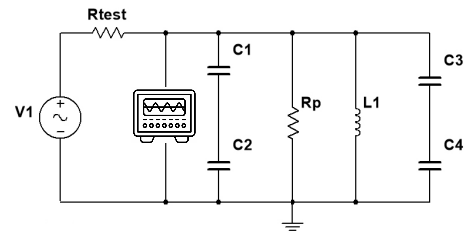
\includegraphics[width=0.8\textwidth]{Imagenes/medicion_rp.png}
    \caption{Medicion de $R_p$}
    \label{fig: de la medicion de la resistencia de perdida}
\end{figure}

Tenemos que colocar la frecuencia del generador de onda en la frecuencia de resonancia $f_o$, ya que la reactancia inductiva y capacitiva se anulan.
Por lo tanto nos quedara la resistencia de test $R_{test} = 1k\Omega$ en serie con la resistencia de perdida $R_p$. Por lo tanto realizando el divisor resistivo:

\begin{equation}
    V_{osciloscopio} = V_{B1} \cdot \frac{R_p}{R_p + R_{test}}
\end{equation}

Y despejando $R_p$ obtenemos:

\begin{equation}
    R_p = \frac{R_{test} \cdot V_{osciloscopio}}{V_{B1} - V_{osciloscopio}}
\end{equation}

Las mediciones son las siguientes:
% Hacer itemize con las mediciones
\begin{itemize}
    \item $V_{osciloscopio} = 2 V$
    \item $V_{B1} = 1.76 V$
    \item $R_p = 7.3 k\Omega$
\end{itemize}

\subsubsection{Medicion de $Z_{in}$}

Para la medicion de la impedancia de entrada, se utiliza el esquema de la figura \ref{fig: de la medicion de la impedancia de entrada}
y la \ref{fig: de la medicion de la impedancia de entrada 2}

\begin{figure}[h]
    \centering
    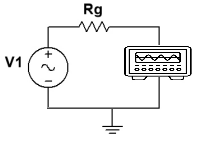
\includegraphics[width=0.8\textwidth]{Imagenes/medicion_zin1.png}
    \caption{Medicion de $V_g$}
    \label{fig: de la medicion de la impedancia de entrada}
\end{figure}

\newpage

\begin{figure}[h]
    \centering
    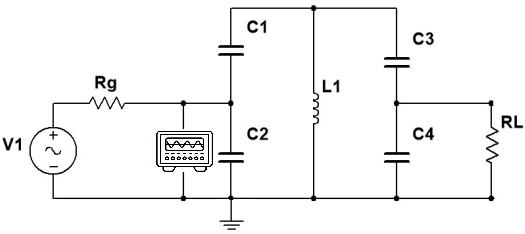
\includegraphics[width=0.8\textwidth]{Imagenes/medicion_zin2.png}
    \caption{Medicion de $V_{in}$}
    \label{fig: de la medicion de la impedancia de entrada 2}
\end{figure}

Con estas dos mediciones podemos calcular la impedancia de entrada. Las mediciones son las siguientes:
% Tabla con mediciones de Vg y Vin
\begin{table}[h]
    \centering
    \begin{tabular}{|c|c|}
    \hline
    \rowcolor[HTML]{C0C0C0} 
    \textbf{Medicion} & \textbf{Valor} \\ \hline
    $V_g$            & 2.3  V         \\ \hline
    $V_{in}$         & 0.7 V         \\ \hline
    \end{tabular}
\end{table}

Debido a que medimos en resonancia, la reactancia inductiva y capacitiva se anulan. Por lo tanto podemos plantear el divisor resistivo:

\begin{equation}
    V_{in} = V_g \cdot \frac{Z_{in}}{Z_{in} + R_{g}}
\end{equation}

Despejando $Z_{in}$ obtenemos:

\begin{equation}
    Z_{in} = R_g \cdot \frac{ V_{in}}{V_g - V_{in}}
\end{equation}

Remplazando los valores obtenemos:

\begin{equation}
    Z_{in} = 22\; \Omega
\end{equation}

\subsubsection{Medicion de $Z_{out}$}

Para la medicion de la impedancia de salida, se utiliza el esquema de la figura \ref{fig: Primer esquema de la medicion de la impedancia de salida} y la figura
\ref{fig: Segundo esquema de la medicion de la impedancia de salida}.

%
\begin{figure}[h]
    \centering
    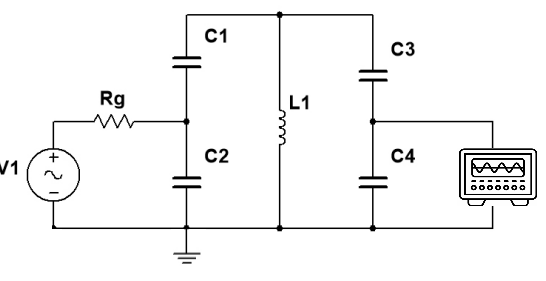
\includegraphics[width=0.8\textwidth]{Imagenes/medicion_zout1.png}
    \caption{Medicion de $V_{out}$ sin carga}
    \label{fig: Primer esquema de la medicion de la impedancia de salida}
\end{figure}

% 
\begin{figure}[h]
    \centering
    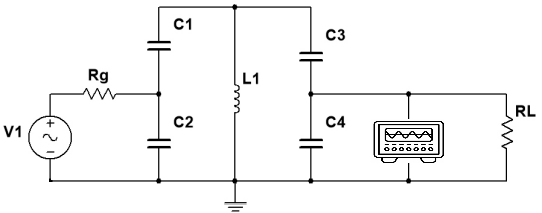
\includegraphics[width=0.8\textwidth]{Imagenes/medicion_zout2.png}
    \caption{Medicion de $V_{out}$ con carga}
    \label{fig: Segundo esquema de la medicion de la impedancia de salida}
\end{figure}




Realizando estas dos mediciones podemos calcular la impedancia de salida. Las mediciones son las siguientes:

% Tabla con mediciones de Vout sin carga y con carga
\begin{table}[h]
    \centering
    \begin{tabular}{|c|c|}
    \hline
    \rowcolor[HTML]{C0C0C0} 
    \textbf{Medicion} & \textbf{Valor} \\ \hline
    $V_{out}$ sin carga            & 1.05  V         \\ \hline
    $V_{out}$ o $V_{L}$ con carga         & 2.4 V         \\ \hline
    \end{tabular}
\end{table}

Planteando el divisor resistivo:

\begin{equation}
    V_{L} = V_{out} \cdot \frac{Z_{L}}{Z_{out} + Z_L}
\end{equation}

Despejando $Z_{out}$ obtenemos:

\begin{equation}
    Z_{out} = Z_L \cdot \frac{V_{out} - V_L}{V_L}
\end{equation}

Remplazando los valores obtenemos:

\begin{equation}
    Z_{out} = 1285\; \Omega
\end{equation}



\newpage
\section{Resultados finales}

En la siguiente tabla se presentan los resultados obtenidos comparado con los valores de diseño: 
% Tabla de resultados donde este en primer columna el parametro, en la segunda el diseño, 3ra valor medido y 4ta error porcentual. Los parametros son 
% frecuencia central L Rp BW Zin Zout Qc Qd
\begin{table}[H]
\centering
\begin{tabular}{|c|c|c|c|}
\hline
\rowcolor[HTML]{C0C0C0}
\textbf{Parámetro} & \textbf{Diseño} & \textbf{Valor medido} & \textbf{Error porcentual} \\ \hline
$f_o$ & 16 MHz & 16.3 MHz & 1.875\% \\ \hline
L & 0.56 $\mu$H & 0.538 $\mu$H & 3.57\% \\ \hline
Rp & 34.3 k$\Omega$ & 7.7 k$\Omega$ & 77.6\% \\ \hline
BW & 1.6 MHz & 1.45 MHz & 9.37\% \\ \hline
Zin & 50 $\Omega$ & 22 $\Omega$ & 56\% \\ \hline
Zout & 1000 $\Omega$ & 1285 $\Omega$ & 28.5\% \\ \hline
Qc & 10 & 11.2 & 12\% \\ \hline
Qd & 610.4 & 139.7 & 77\% \\ \hline
\end{tabular}
\caption{Resultados obtenidos}
\label{tab:resultados}
\end{table}





\newpage
\section{Conclusiones}

En este trabajo se diseñó y construyó un circuito resonante, aplicando conceptos abordados en clase. El resultado de los cálculos y las mediciones no son 
exactamente iguales debido a múltiples factores.


El principal inconveniente a la hora de realizar el armado del circuito es el inductor. Para empezar, a la hora de comprar cobre para realizar el inductor,
no sabemos si el cobre es puro o no, lo que afecta a la resistencia del inductor. Por otro lado, al bobinar a mano el inductor, no tenemos la certeza de que 
la separación entre espiras sea la misma en todo el inductor, y además el cobre al tener un grosor de $2.1 \, \text{mm}$, no se puede bobinar de manera perfecta ya que 
este tiende a deformarse, lo que afecta a la inductancia del inductor. Al cambiar la inductancia, cambia la frecuencia de resonancia, lo que hace que la adaptación
de impedancias necesite otros valores de capacitores. Otro problema que tuve fue que al realizar las mediciones en dos días distintos,
los valores de las mediciones no eran iguales, lo que me llevó a tener que realizar las mediciones nuevamente. Esto se debió a que al transportar el circuito, lo modifiqué
levemente. También puede deberse a que utilicé un osciloscopio distinto, lo que puede afectar a las mediciones.


Observando la tabla de resultados, podemos ver que en $R_p$ el error es del $77.6\%$. Los cálculos realizados de la resistencia de pérdidas son de $34.3 \, \text{k}\Omega$, mientras
nosotros medimos $7.7 \, \text{k}\Omega$. Esto provocará que la potencia transferida sea menor debido a que el circuito no se encuentre adaptado. Esto se refleja en las 
mediciones de $Z_{\text{in}}$ y $Z_{\text{out}}$, donde los valores medidos no son iguales a los valores de diseño. En $Z_{\text{in}}$ el error es del $56\%$ y en $Z_{\text{out}}$ el error es del $28.5\%$.


Los capacitores utilizados son capacitores de cerámica, que cuentan con una tolerancia del $-20\%$ al $80\%$. Esto afecta a la frecuencia de resonancia y además a la adaptación
de impedancias. 


Otro problema que afecta radicalmente las mediciones son los instrumentos de medición. En este caso, aunque utilizamos conectores BNC,
se agrega la capacidad parásita de los cables, del mismo osciloscopio y del generador de señales. 



La solución al problema del trabajo artesanal del inductor es utilizar un bobinador de inductores, que nos permita bobinar inductores de manera más precisa. Utilizar calibre 
para ajustar, si es necesario, la distancia entre espiras. Esto nos permitirá tener una inductancia más precisa y una resistencia de pérdidas más cercana a la calculada.
Otra solución es utilizar inductores comerciales, que cuentan con una inductancia y resistencia de pérdidas específica. Además, para mejorar la adaptación de impedancias
podrían utilizarse capacitores de poliéster de $1\%$ de tolerancia, aunque encarecería el trabajo práctico. Y la última mejora podría ser utilizar un osciloscopio 
de alta frecuencia y un generador de señales de alta frecuencia, para disminuir la capacidad parásita de los cables y de los instrumentos de medición. Además, para medir 
la adaptación de impedancias, podría utilizarse un roímetro, que nos permitiría medir la potencia transferida y así saber si el circuito se encuentra adaptado o no.



Finalmente, considerando los problemas anteriormente mencionados y las soluciones propuestas, el trabajo nos permite tener un mayor entendimiento de los circuitos resonantes,
y además poder observar el efecto de las altas frecuencias en los circuitos.

\newpage
\printbibliography
\end{document}